\documentclass[output=paper]{LSP/langsci} 
\ChapterDOI{10.5281/zenodo.1441345}

\author{Maria del Mar Vanrell\affiliation{Universitat de les Illes Balears}\and
Ingo Feldhausen\affiliation{Goethe-Universität Frankfurt am Main}\lastand
Lluïsa Astruc\affiliation{The Open University}
}

\title{The Discourse Completion Task in Romance prosody research: Status quo and outlook} 
\shorttitlerunninghead{The Discourse Completion Task in Romance prosody research} 
 
\abstract{The growing interest in the interfaces of prosody with other areas, notably pragmatics, has led to an interesting cross-fertilization of methods such as the \textit{Discourse Completion Task} (DCT). In this chapter, we review previous and ongoing work in which the DCT method has been used to research Romance prosody. First, we introduce the design of the DCT used in pragmatics. After that, we discuss the design of the DCT used in Romance prosody and examine the strengths and weaknesses of the DCT method. Finally, we propose modifications and show how the DCT method can be further strengthened. All in all, we conclude that the DCT is an adequate method to research Romance prosody (as well as the prosody of other languages) and that future research should continue to consider how to further refine and improve this data collection instrument.}

% \textbf{Keywords:} Discourse Completion Task, Romance prosody research, questionnaires, reliability, validity, modifications of the classical design of DCT


\maketitle
\begin{document}
\label{chap:van}\label{ch:6}

\section{Introduction}
\label{sec:van:1}
The Discourse Completion Task (henceforth DCT) is a relatively new method in prosodic research adopted from the field of pragmatics, where it has been used for decades for both research and assessment. Due to the numerous advantages of this method (see \sectref{sec:van:2} below for details), the DCT has found a place in the field of prosody. It is time now to take a step back and assess the strengths and weaknesses of the DCT before considering how it can be improved and strengthened in future studies. 

\subsection{Research paradigms in empirical research in prosody}
\label{sec:van:1.1}
To place the DCT within the repertoire of empirical methods available in prosody, we need to imagine a hypothetical continuum of varying degrees of researcher interference ranging from correlational to experimental research (see \figref{fig:van:1}).\footnote{Different criteria can be used to classify the methodological approaches to prosody research. For instance, \citet{Niebuhr2015} propose the following five dimensions: (i) degree of control over experimental variables (which broadly corresponds with the proposal defended in this paper), (ii) event density or the number of tokens per time unit, (iii) expressiveness, (iv) communicative intention, and (v) homogeneity of behavior.} The DCT would find its place in the middle of this continuum. 
% % \todo{tikz?}
\begin{figure}
% [Warning: Draw object ignored]
\begin{tikzpicture}[row 1/.style={font=\bfseries\sffamily},font=\sffamily]
\matrix (vanfig) [draw,matrix of nodes,nodes in empty cells] {
  Correlational research & & Experimental research\\
  & Researcher interference & \\
  − & & +\\
  \\
  Corpora & Self-report responses\slash questionnaires & Experiments\\
};
\draw[<->,thick,dashed] (vanfig-3-1) -- (vanfig-3-3);
\foreach \x in {1,2,3} {\draw[->,thick] (vanfig-5-\x) -- (vanfig-3-\x);}
\end{tikzpicture}
\caption{Diagram illustrating the continuum between correlational and experimental research.}
\label{fig:van:1} 
\end{figure}

As we see in \figref{fig:van:1}, empirical research in prosody encompasses both correlational and experimental research. The difference between these types of research is that in correlational studies the researcher observes what naturally goes on in the world with little or no direct interference by the researcher. S/he tries to determine if a relationship or covariation exists between two variables, such as different types of intonational patterns and different dialects, for example. Experimental research, in contrast, aims to isolate cause and effect by manipulating one or more variable/s to assess the effect of such manipulation on another variable, the dependent variable. 

In the continuum shown in \figref{fig:van:1}, corpora composed of spontaneous speech would occupy the left-hand end, which would also correspond to the most ecologically valid data.\footnote{Ecological validity refers to an experimental condition in which the methods, the materials and the setting are as natural as possible, that is, close to the real world.} Some of the speech corpora used in prosody research are the ICE-GB corpus (\citealt{Wichmann2003}), the Boston database of FM radio news speech (\citealt{Ostendorf1995}), the CALLHOME corpus \citep{Ogden2006}, the Spontal corpus (\citealt{Edlund2010}) and the Map Task corpus \citep{Anderson1991}. For Romance languages specifically, we should mention the ESTER corpus for French media speech (\citealt{Gravier2004}), the corpus of casual French (\citealt{Torreira2010}), the Glissando corpus \citep{Garrido2013Glissando} for Catalan and Spanish and the Val.es.co corpus (\citealt{CabedoNebot2013ValEsCo}) for Spanish (for further details see \citealt{Delais-Roussarie2008,Post2012,Delais-Roussarie2014}). 

The use of large corpora in prosody research has had an effect on other research in the development of speech processing software, statistical procedures to assess the reliability of auditory analyses, and the development of online tools for sharing data with the research community and general public. One of the outcomes of research using large corpora is the development of automatic procedures to detect prominence, phrase boundaries and tonal events (that is, peaks and valleys), such as Analor (\citealt{Avanzi2010}), ModProso, SegProso (\citealt{Garrido2013ModProso,Garrido2013SegProso}) or the ProsodyDescriptor \citep{Barbosa2013}. Different tests have been proposed to assess intertranscriber reliability such as the pairwise transcriber agreement and the kappa statistic (Cohen kappa and Fleiss kappa)  (\citealt{Brennan1981,Yoon2004,Randolph2008,Mo2008,Escudero2012}, among others). 

New tools have also been developed to make corpora available on the Internet. One of the most recent such projects in the field of Romance intonation is the \textit{Interactive Atlas of Romance intonation} (\citealt{Prieto2010.2014.Atlas}). The \textit{Atlas} uses interactive maps of Europe and the Americas to display audio and video data collected using a Map Task and a questionnaire in the form of a DCT (see discussion below). The \textit{Atlas} follows a line of research that has a long tradition within Romance linguistics (\citealt[55]{Geckeler2003}). These \textit{language atlases} mainly concentrate on segmental phonetics and phonology, morphology, and the lexicon, and date back to the \textit{Deutscher Sprachatlas} (DSA, Georg Wenker 1876--1888 in Germany) and the \textit{Atlas linguistique de la France} (ALF, \citealt{Gillieron1902–1910}); see \citet{Goebl1992} or \citet{Auer2010} for an overview. At the end of the last century, these atlases also started to appear in digital form (e.g. \citealt{Goebl1998,Kattenbusch1998-2016}). The recent technological revolution has resulted in the widespread availability of devices and software to collect and display data. As a consequence, it is easier for language atlases to include spontaneous speech. A challenge for future research would be to combine different types of atlases in order to provide linguistic information from different linguistic modules in one and the same interactive atlas.

At the other end of the continuum lies experimental research (see \figref{fig:van:1}). As discussed above, experimental research involves the manipulation of a variable or variables to measure their possible effect upon another variable, the dependent variable. Some common dependent variables used in experimental research are behavioral measures and physiological responses. In behavioral experiments responses are produced automatically, without conscious thought. Participants typically sit at a computer where they receive visual or auditory stimuli and press buttons in response.\footnote{This is a very general definition that includes different types of behavioral experiments (please see \citeauthor{GiliFivela.2018}, this volume, for a more precise classification).} The researcher then counts the number of times a particular response occurs. Within this approach in prosody, we find paradigms such as the Categorical Perception paradigm  (e.g. \citealt{Kohler1987,Ladd1997,Chen2003,SchneiderEtAl2006,Feldhausen2011,Vanrell2011}), the Gating paradigm (e.g. \citealt{Hadding-Koch1964,Heuven2002,Vion2006,Face2007,Petrone.2011,Crespo-Sendra2011}, among others), the imitation task (\citealt{Pierrehumbert1989,Dilley2005,Dilley2007,Vanrell2011}), and the Priming paradigm (\citealt{Cutler1986,Jun2015}) (all used with adults) or the Head-turn preference procedure (\citealt{Jusczyk1993}) (used mainly with children of 6--12-months old). 

Sometimes these paradigms can also be combined with reaction time measurements (\citealt{Chen2003,Feldhausen2011}), i.e. the speed with which someone reacts to a stimulus. Examples of physiological responses include acoustic (F0, local or global duration) and articulatory analyses of speech productions (see \citealt{Prieto1995,Arvaniti1998,Frota2002} for acoustic and articulatory analysis; and see \citealt{DImperio.2007,Muecke2006,Stella2014} and \citeauthor{GiliFivela.2018}, this volume, for articulatory analyses). Of particular interest are methods which have been applied only recently to prosody research and which measure brain activity (Event Related Potentials (ERPs) and Brain Imaging Techniques (fMRI); see \citealt{Kaiser2006} for details) and patterns of attention in babies and adults (Eye-tracking paradigm; see \citealt{Watson2006} for details). For an overview of the experimental methods and paradigms for prosodic analysis see \citet{Sudhoff.2006}, \citet{Prieto.2012}, and \citet{Niebuhr2015}, among others. Differences between read and spontaneous speech are addressed in \citet{Llisterri1992,Beckman1997,Face2003,Xu2010}, and \citet{Wagner.2015}, among others. A comprehensive overview of research methods in linguistics from a more general point of view, including experimental methods, is provided in \citet{Podesva.2013}.

Halfway between correlational and experimental research are self-report responses and questionnaires (\figref{fig:van:1}), and among these, the DCT. These methods have been borrowed from research in pragmatics, where they have been commonly used to research and assess language learners’ pragmatic development. Self-report responses/questionnaires typically take the form of a survey or questionnaire in which the respondents read the questions and select a response based on their attitudes or beliefs. Researcher interference can be regarded as medium, since some variables can be tightly controlled but the respondents still have the freedom to answer in a very natural way. According to \citet{kasper2002}, three different categories can be distinguished: oral and written self-reports, measures of spoken interaction, and questionnaires. 

\textbf{Oral and written-self reports} can be further classified into interviews, think-aloud protocols and diaries (less commonly used). Interviews are used to tap into ``the participants’ long-term memories of generalized knowledge states, attitudes or past events” (\citealt[107]{kasper2002}). Think-aloud protocols basically require participants to verbalise their thinking processes as they are performing a specific task. They can take place simultaneously with a DCT, for example, but they can also be used retrospectively (\citealt{Cohen1993,Robinson1992}). They can also be audio- or video-recorded.  

Regarding \textbf{measures of spoken interaction}, an important distinction should be made between elicited conversations and role-plays. In elicited conversations the participants do not take on roles different from their own, whereas in role-plays they are asked to take on specified roles (\citealt{kasper2002}). By adopting different roles, the influence of power, distance and degree of imposition (\citealt{Brown1987}) that motivate specific linguistic choices can be explored.

Three different types of \textbf{questionnaires} can be distinguished: DCT, multiple choice questionnaires and scaled-response formats. In DCTs, participants are presented with short (usually written, although not necessarily) role-plays based on everyday situations designed to elicit specific speech acts. They are required to complete a turn of dialogue for each item \citep{Barron2003}. Multiple choice questionnaires present items containing a question and different alternatives, from which the participants must choose the most appropriate one. These questionnaires are often used to gather information about pragmatic production and comprehension  (\citealt{kasper2002}). In scaled-response formats, the participants judge the degree of appropriateness (also the degree of power, distance, imposition, etc.) of a particular item in a specific context using a Likert scale.

\subsection{The \textit{Discourse Completion Task} in research on pragmatics}
\label{sec:van:1.2}
A DCT is defined as a questionnaire which can be administered either orally or in writing and describes different scenarios designed to elicit the desired speech act. Informants respond by completing a turn of dialogue (\citealt{Kasper1991,Brown2001}). What sets this methodology apart from other contextualized elicitation tasks is that the prompt usually contains not only foreground and background information about the current event but also information on the social distance between the interlocutors. Typically, five different types of DCT are distinguished \citep{Nurani2009}. In the classic format, the prompt finishes with a reply, whereas in the second type, the dialogue is initiated by the interlocutor and no reply is offered (see \REF{ex:van:1} and \REF{ex:van:2}, respectively). In the third type, there are neither interlocutor initiations nor replies, and participants are completely free to respond however they wish, though they must give a verbal response (the \textit{open item-verbal response only construction}, see \REF{ex:van:3}). In the fourth format, the \textit{open item free response construction} (see \REF{ex:van:4}),  participants can give either a verbal or a non-verbal response, or even no response at all. The fifth type is similar to the open item-verbal response format, but includes detailed situational background (see \REF{ex:van:5}); both an old and a new version exist, which differ in the details given in the prompt. 


\ea
    \label{ex:van:1}
\textit{Classic format:} Walter and Leslie live in the same neighborhood, but they only know each other by sight. One day, they both attend a meeting held on the other side of town. Walter does not have a car but he knows Leslie has come in her car.


Walter: {\longrule\longrule\longrule\longrule\longrule\longrule\longrule}

Leslie: I’m sorry but I’m not going home right away.

  (\citealt{BlumKulka1989})
\z

\ea%2
    \label{ex:van:2}
 

          \textit{Dialogue construction}: Your advisor suggests that you take a course during summer. You prefer not to take classes during the summer. 

Advisor: What about taking a course in the summer?

You: {\longrule\longrule\longrule\longrule\longrule\longrule\longrule}

(\citealt{Bardovi-Harlig1993})

    \z
\ea%3
    \label{ex:van:3} 
          \textit{Open item-verbal response only:} You have invited a very famous professor to an institutional dinner. You feel extremely hungry, but someone starts speaking and nobody has started eating yet, because they are waiting for the guest to start. You want to start having dinner. What would you say?

\citep{Safont-Jorda2003}

    \z

\ea%4
    \label{ex:van:4} 
          \textit{Open item free response construction:} You are the president of the local chapter of a national hiking club. Every month the club goes on a hiking trip and you are responsible for organizing it. You are on this month’s trip and have borrowed another member’s hiking book. You are hiking by the river and stop to look at the book. The book slips from your hand, falls in the river and washes away. You hike on to the rest stop where you meet up with the owner of the book.

You: {\longrule\longrule\longrule\longrule\longrule\longrule\longrule}

(\citealt{Hudson1995})
    \z


\ea%5
    \label{ex:van:5} 

          \textit{Old version:} A student in the library is making too much noise and disturbing other students. The librarian decides to ask the student to quiet down. What will the librarian say?

(\citealt{Billmyer2000})

\textit{New version:} It is the end of the working day on Friday. You are the librarian and have been working in the University Reverse Room for two years. You like your job and usually the Reverse Room is quiet. Today, a student is making noise and disturbing other students. You decide to ask the student to quiet down. The student is a male student who you have often seen work on his own in the past two months, but today he is explaining something to another student in a very loud voice. A lot of students are in the library and they are studying for their midterm exams. You notice that some of the other students are looking in his direction in an annoyed manner. What would you say?

(\citealt{Billmyer2000})
    \z

DCT methods have a long history in pragmatics, and though their reliability and validity have been the subject of much discussion in this field, they have yet to be reviewed in the field of prosody. According to \citet{Nurani2009} and \citet{Cyluk2013}, some of the strengths of this method for pragmatics research include the possibility of collecting a large amount of data in a short time, the control of contextual variables and demographic information, and the possibility to compare two or more languages. Compared to natural speech, the use of a DCT elicits a prototypical response, whereas natural data is more likely to trigger less common items \citep{Kwon2004}. Researchers have also argued that DCT methods are limited in terms of the authenticity of the situations, with interactions being much simpler than in real conversations and with responses to the scenarios that may not correspond with what speakers would actually say in real life. Additionally, it has been noted that traditional written DCTs used in pragmatics research do not collect or analyze the use of non-verbal features such as gestures or facial expressions, as well as paralinguistic elements such as pitch and intonation (\citealt{Cyluk2013}, which in turn cites \citealt[326]{Kasper2000}). Scholars seem to agree that the validity and reliability of this method should be evaluated in terms of the objectives of the investigation. Thus, the DCT is an effective method when the aim of the study is “to inform about the speakers’ pragmalinguistic knowledge of the strategic and linguistic forms by which communicative acts can be implemented, and about their sociopragmatic knowledge of the context factors under which particular strategies and linguistic choices are appropriate” \citep[329]{Kasper2000}, but should be avoided if the focus is on conversational interaction.

Acknowledging that the DCT has, as does every data collection method, advantages and disadvantages, scholars have focused on possible ways to strengthen the design of a typical DCT. Possibilities range from enriching the contextual detail of DCT prompts (\citealt{Billmyer2000,Rose2000,Cohen2003,Schauer2004,McLean2005}, among others) to the use of two or more methods (triangulation) \citep{Wiersma1986} to verify the validity of the data while reducing possible task bias.

In this chapter we will review previous and ongoing work in which the DCT has been applied to Romance prosody. First, we will analyze the design of DCTs applied to this field, before examining their strengths and weaknesses while considering their reliability/validity. Finally, we will discuss some of the modifications proposed in the literature and suggest a few other improvements.  

\section{Use of the DCT in Romance prosody research}
\label{sec:van:2}
In this section, we review some of the studies that have applied the DCT to Romance prosody as a data collection instrument. In doing so we highlight the strengths and weaknesses attributed to the DCT in these studies and add considerations of our own. We do not intend to offer an exhaustive literature review, which would be impossible, given the increasing popularity of this method in this field. Rather, we will concentrate on studies that clearly address issues regarding the validity or reliability of the method. \tabref{tab:van:1} provides the reader with a summary of the method’s strengths and weaknesses explored in this section.

\begin{table}
\begin{tabularx}{\textwidth}{XX}
\lsptoprule
 \bfseries Strengths & \bfseries Weaknesses\\
 \midrule
Collection of large amount of data within a short period of time. & Situations not always easily to understand (which may lead to rising contours meaning “Did I do it well?” or to contours expressing obviousness).\\
\tablevspace
Elicitation of comparable (semi-) spontaneous data across speakers and varieties. & The intonational patterns obtained may not always coincide with those previously found.\\
\tablevspace
Feasible for older and illiterate people. & Elicitation of less trivial speech acts can be difficult.\\
\tablevspace
Little and easily transportable recording equipment is required. & Cultural differences or social / psychological factors may arise.\\
\tablevspace
Control of both the context (pragmatic and politeness factors) and relevant aspects of the target sentence (stress pattern, sentence type and segmental and syntactic structure). & The range of situations may not portray the variety of language uses in real situations.\\
\tablevspace
Interface phenomena (such as syntax and prosody, word order and information structure or pragmatics, etc.) can be easily addressed. & The DCT does not allow for scripted speech (and thus cannot easily address research questions that need predetermined answers).\\
\tablevspace
The task can be used for studies on monolingual speakers (L1) and (different types of) bilingual speakers (L2, 2L1, eL2, heritage speakers...). & Each context allows for only one answer; it is not possible to assess how felicitous other sentences would be in the same context.\\
\tablevspace
Allows the speaker to freely utter any response as long as it fits the situation evoked by the prompt. & Establishing different contexts may be difficult in case in which the pragmatic differences between contexts are unclear.\\
\lspbottomrule
\end{tabularx}
\caption{\label{tab:van:1} Main strengths and weaknesses attributed to DCT used in the context of Romance prosody.}
\end{table}

The DCT has been applied to different fields of research on Romance prosody such as intonational phonology (\citealt{Prieto.2001,Prieto2007-2012,Prieto2010,Prieto2009-2013,Brehm2014,Frota2015romance,Roseano2015preguntas,Huttenlauch2016}), language contact (\citealt{Sichel-Bazin2015}), L2 acquisition (\citealt{Craft2015,Astruc2016politeness}), sociophonetics (\citealt{Mascaro2015}), prosody and its interfaces (\citealt{Vanrell2014dialectinterrogatives,Vanrell2014sardinianpolar,Vanrell2014evidentiality,ElviraGarcia2017,SanchezAlvarado.2018,Huttenlauch.accepted}), Politeness theory (\citealt{Astruc2011,Astruc2016politeness,Borras-Comes2015}) and visual prosody (\citealt{Cruz2015,Gonzalez-Fuente2015}; \citeauthor{GiliFivela.2018}, this volume). The Romance languages explored through the use of this method include Catalan, French, Friulian, Italian, Occitan, Portuguese, Romanian, Sardinian and Spanish. 

As far as we know, the DCT was first applied to Romance prosody research by \citet{Prieto.2001}, who worked on the intonation of absolute questions in different varieties of Catalan. Later on, the DCT was used by \citet{Prieto2007-2012} to collect data for the \textit{Interactive Atlas of Catalan intonation}. According to the authors and collaborators of the \textit{Interactive Atlas of Catalan Intonation}, one of the clear advantages of using this method is that it allows the researcher to collect semi-spontaneous speech within a short period of time, while still controlling for the stress pattern (stress on the penultimate or antepenultimate syllable) of the last word in the utterance, segmental structure (use of sonorants), and sentence type of the target utterances. The questionnaire was designed to elicit different sentence types (statements, questions, commands and requests, and vocatives), which contained mostly voiced segments so that the resulting F0 contour was generated with no interruptions (i.e., \textit{Sí, dona, d’en Jaume!} ‘Obviously! It’s Jaume’s!’). In addition, the last word of the utterance always contained the stress on the penultimate or antepenultimate syllable (to provide more room for tonal realization). It was administered orally to 145 females aged between 20 and 45 coming from 70 different Catalan locales from distinct dialectal areas (Alguer Catalan, Balearic Catalan, Central Catalan, Northwestern Catalan, Northern Catalan and Valencian). Importantly, the questionnaire was adapted to each dialect and the researcher administering the questionnaire was a native speaker of the dialect under investigation. The researcher explained each context to the participant. After the participant produced the sentence, the researcher checked whether the utterance agreed with the proposed utterance type and intention. Most of the situations were of the \textit{open item-verbal response only} type (see Introduction), although in some cases the informant was provided with an interlocutor initiation and, in one specific case, with a picture. Until then, the data collection instruments used in Romance prosody research consisted either of read speech or tasks designed to elicit spontaneous speech such as the Map Task methodology (see \citealt{Grice2003}, among others). In this way, the DCT developed for the \textit{Interactive Atlas of Catalan Intonation} constituted a significant improvement in data collection in Romance and has prompted a variety of studies to follow the same approach  (\citealt{Prieto2010,Brehm2014,frotaPrieto2015,Sichel-Bazin2015}). 

Other merits attributed to DCT by \citet{Sichel-Bazin2015} include allowing for the elicitation of comparable spontaneous data across speakers and varieties, its feasibility for older and illiterate people (since the questionnaire was administered orally) and its minimal requirements in recording equipment. \citet{Sichel-Bazin2015} investigated the consequences of language contact on the prosody of Occitan and French. Given the objectives of the project as well as the need to consider the precarious sociolinguistic situation of Occitan, the data collection instrument needed to meet a number of conditions: it should elicit comparable spontaneous data across speakers and varieties, it should be feasible for older and illiterate people, and it should allow the researcher to obtain as many different intonational contours as possible. In addition, Occitan speakers should preferably be recorded at their homes, where they would feel comfortable speaking the language. Easily transportable recording equipment would be required for this purpose. One of the methodologies used was a DCT questionnaire that consisted of 29 situations with different semantic and pragmatic meanings. This was administered to 81 speakers of Northern French, 95 speakers of Southern French and 83 speakers of Occitan. The use of the DCT allowed for the time-efficient collection of data from older participants in their own homes. Some of the problems encountered by the researchers were general issues arising due to the environment in which the survey was conducted: interruptions by people coming into the room where the recording was made or other noises in the homes of the speakers. 

This data collection method enables the researcher not only to control the pragmatic structure (polarity, speaker bias towards the proposition and politeness factors) of the context but also the syntactic pattern (clause type or type of verbs or subjects) of the target sentence. \citet{Vanrell2014dialectinterrogatives} investigated how prosody interacts with word order in the expression of interrogativity in different varieties of two Ibero-Romance languages, Catalan and Spanish. One hundred and thirty questionnaire items were designed by controlling factors of the target sentence such as the type of interrogative (direct/indirect polar and wh-questions), type of verb (copulative, transitive, unaccusative and unergative), type of subject (nominal, pronominal or the second person formal \textit{vostè/usted}), degree of presupposition (information- and confirmation polar questions, and tag questions) and the presence of external interrogative adverbials of the type \textit{how come} (\citealt{Rizzi2001}). The questionnaire was administered to 14 informants from different Catalan and Spanish dialectal areas. One of the clear strengths of this method is that it can reconcile the two perspectives, prosodic and syntactic, when dealing with dialectal variation. In \citet{Vanrell2014sardinianpolar}, the interplay between lexicon, syntax, intonation and pragmatics in Sardinian polar questions was investigated. A questionnaire containing 10 items was designed in which three different bias conditions (neutral, epistemic and evidential) with positive and negative polarities (conveying the speaker bias towards either a positive or negative answer) were manipulated. Neutral situations were not biased towards a positive or a negative response. In the epistemic situations, “the speaker’s bias was based on beliefs or expectations or what s/he would assume to be a norm”, whereas the evidential situations “were based on evidence available in the immediate context of the conversation” \citep[4]{Vanrell2014sardinianpolar}. Eleven Sardinian female speakers, aged between 47 and 73, participated in the task. 

DCT methods have also been used to research politeness intonation (see an introduction to Politeness Theory in \citealt{Brown1987}; see also \citealt{Astruc2011,Astruc2016offers,Borras-Comes2015,Astruc2016offers}). \citet{Astruc2011} and \citet{Astruc2016offers} examined how politeness in offers and requests is encoded by intonation in Central Catalan, a language with two distinct intonational contours for unbiased polar questions. The DCT method permitted the manipulation of social distance, power and the cost of the face-threatening act -- the contextual variables identified as relevant in politeness research -- in two steps: high versus low social distance, high versus low power difference, and high versus low cost. Sixteen scenarios were included in the questionnaire. The carefully controlled design allowed the researchers to conclude that the cost of the act determines the choice of intonation, whereas the power differential between participants may not be a relevant factor. The lack of statistically significant results in the case of the power differential variable could be due to the specific scenarios selected. Specifically, the authors state that “the high power scenario in the DCT presented a work-related situation in the public services context, which may have been interpreted by participants as less face-threatening than expected” (\citealt[110]{Astruc2016offers}). Therefore, a clear strength of the DCT is the possibility to manipulate the social variables relevant to politeness in two or more steps, whereas a drawback can be that designing effective scenarios requires thoughtful consideration and some degree of trial and error.

The findings in \citet{Astruc2016offers} are consistent with those in \citet{Astruc2016politeness}, in which the DCT was applied to the field of L2 acquisition with the aim of comparing the interaction of politeness and intonational phonology in first and second language. The DCT questionnaire was used to elicit spoken data from 12 speakers of Mexican Spanish. The questionnaire contained 16 scenarios, of which eight were offers and eight requests, and controlled for social distance, the power of the hearer over the speakers and the cost of the face threatening act. Participants completed the survey three times. The first time they were asked to say anything they would say in a real situation. The second time they had to ask a question, while the third time they were asked to imagine that the hearer rejected their request (this last part has yet to be analysed). The rationale for a free response followed by a sentence-only response is to allow participants to immerse themselves in the scenarios, which should thus elicit responses that are more natural and appropriate to the context. Again, power was not found to be a relevant factor and the authors hypothesize that this may be due to changing conditions in the Mexican workplace (also confirmed by some participants): “[...] they commented in their interviews on the new tendency in the private sector to treat everybody as an equal (“no rank: we are a team”). In the public sector, differences in rank are felt to be more marked and people address each other using titles such as \textit{licenciado} or \textit{ingeniero} (ʽgraduateʼ and ʽengineerʼ, respectively)” (\citealt[22]{Astruc2016offers}). 

\citet{Borras-Comes2015} investigated the pragmatic conditions underlying the choice of three vocative pitch contours in Central Catalan. The DCT allowed them to manipulate other relevant contextual variables such as physical distance and the insistence of the call, in addition to power and social distance. Their questionnaire contained 16 scenarios, and 20 participants (17 females and three males) took part in the experiment. The results obtained through the DCT questionnaire were complemented by an acceptability judgment task. A perception test was needed to confirm the results of the DCT data, as with this method “each participant could only produce one contour for a given communicative context, meaning that this methodology does not allow us to adequately assess how felicitous other possibilities would be in that specific context” (\citealt[74--75]{Borras-Comes2015}).\largerpage[-1]

In terms of weaknesses of the DCT, some authors (\citealt{Sichel-Bazin2015,Vanrell.unpublished,Vanrell2014sardinianpolar}) note that speakers may struggle to understand the task, possibly giving rise to the use of rising contours meaning “Did I do it well?” or expressing obviousness. This latter effect has also been reported by \citet{Vanrell.unpublished} as a task-induced effect. According to them, through this final rise the participants might manifest their perplexity at having to reply to questions whose answers are evident from the visual stimuli used in their elicitation task.

Other scholars such as \citet{Uth2014} had already recognized potential problems with the use of images to elicit language production. Asking the participants about what they see in the images can favor the marking of evidentiality (referring to a visual source of information) and also epistemicity (given that the answer is evident from the pictures). Following the same line of reasoning and according to personal communication with Francesc Ballone (28.09.2016), some of the questionnaire items used in \citet{Vanrell2014sardinianpolar} represented a challenge for the speakers in that they were very long and sometimes contained very specific details that might easily go unnoticed (see \ref{ex:van:6}).

\ea%6
    \label{ex:van:6}

         The city council has published a very nice booklet about the history of the Santu Pedru in Vincoli church and it is being distributed free of charge. A neighbor of yours goes to the city council to get one of them and you ask her to pick one up for you too. The problem is that sometimes she forgets things. When you see that she’s coming back, ask her whether she’s bringing one for you, presuming that she probably isn’t.
    \z

There have also been concerns regarding the fact that the intonational patterns obtained through this method may not always coincide with those found in previous investigations using different methodologies. For instance, the nuclear patterns found in Italian yes-no questions are shown in Figure 5.10 in \citet[169]{GiliFivelaETAL2015intonationalvariation}. The authors note that the patterns evident in this figure did not always coincide with those found in previous investigations in which a different methodology was used (i.e. Map Task dialogues). They attribute this difference to the elicitation method, which may induce “different types of assumption concerning the knowledge shared by the possible interlocutors” in the speakers \citep[168]{GiliFivelaETAL2015intonationalvariation}. It is also noted in \citet{Vanrell2014dialectinterrogatives} that the intonational results for Castilian Spanish yes-no questions do not conform with the predictions made by traditional studies such as \citet{NavarroTomas.1944} and \citet{Quilis1981}, since the expected intonational pattern for Castilian Spanish yes-no questions would be L* H\% rather than L+¡H* L\%. However, it is interesting to note that Vanrell \& Fernández-Soriano’s findings do agree with those of \citet{Henriksen2016}, in which polar questions uttered in spontaneous speech are analysed. The authors argue that a possible explanation for this inconsistency could be that L* H\% contours are more common in formal speech situations (\citealt{Henriksen2013,Henriksen2016}).

While the previous sections have mainly summarized comments on the \linebreak strengths and weaknesses found in the literature, we would like to add additional considerations in what follows. In using DCTs in our research we have noticed some problems that must be addressed.

First, in order to elicit different speech acts, both the interviewer and the participant must establish a certain degree of participation. When reading the situation/context for a simple statement and uttering a corresponding response, neither the interviewer nor the participant need to expend much effort. However, when the speech act is less trivial, such as in the case of counterexpectational or rhetorical questions, the task is more complex for both participants. A counterexpectational question, for example, hinges on the fact that the participant utters the question with a certain degree of surprise. Consequently, it is important that the participant fully understands each scenario. In the questionnaires for the Intonation Atlases, for example, many different situations appeared one after another and the participant must get into the spirit of each new situation immediately.

Second, even if there is no rapid change between the different situations, a specific situation can still be challenging due to cultural circumstances. In their study on imperatives in Mexican Spanish, \citet{Brehm2014} created situations evoking short and long imperatives (imperatives consisting of one word, i.e. the verb, and imperatives consisting of the verb followed by an argument). All participants had initial difficulties in uttering imperatives, commenting that imperatives are considered to be very impolite and, as such, are seldom used. Thus, instead of saying \textit{¡Dímelo!} ‘Tell me that!’, the speakers seemed to prefer using an absolute question combined with the conditional, i.e., something like \textit{¿Podrías decirmelo?} ‘Could you tell me that?’.\footnote{These observations match the results presented in \citet{BlumKulka1989}, which demonstrate that different languages may use varying sentence types (imperatives, indirect requests, hints) to produce requests.} The authors then asked participants to ignore politeness conventions and reply using only imperatives. Thus, in addition to using the variety-specific lexicon (as mentioned above), researchers should also be aware of culture-dependent rules of politeness and other social factors. Furthermore, psychological factors such as introvert/extrovert, expressive/inexpressive, etc. as well as gender differences between the interviewer and the interviewee may also play a role (see a discussion about participant selection in \citealt[22--23]{Niebuhr2015}).

A third difficulty in setting up a successful DCT is that of establishing clear pragmatic boundaries between the different scenarios. While the difference between a neutral statement and a neutral wh-question or a vocative may be intuitively clear, the difference between different types of wh-questions (such as neutral and counterexpectational echo wh-questions; see, e.g., \citealt{Huttenlauch2016}) may not. For this reason, it is necessary to clearly define the pragmatic context most likely to elicit each intended speech act and to design each scenario according to these definitions.

A standard question in experimental research is how to proceed when par\-ti\-ci\-pants do not behave as expected: 

(a) A participant may not understand a given scenario, and thus cannot provide a pragmatically appropriate response. If this concerns only one or two participants, their data can be withdrawn from the experiment. If this applies to the majority of the par\-ti\-ci\-pants, however, the scenario might not be optimal and needs to be revised. 

(b) A participant might give a non-corresponding answer, such as uttering \textit{¿Podrías decirmelo?} ‘Could you tell me that?’ in a scenario which should elicit an imperative. In this case the interviewer might intervene and ask for the intended speech act. As described above, this can be more or less difficult.

(c) A participant may have replied adequately to the situation, but in doing so adds further material. An imperative, for example, could be followed by the interjection \textit{por favor} ‘please’, as in the following Spanish example: \textit{Mírala, por favor.} ‘Please look at her’. Now the question arises as to whether the interjection can be discarded from the analysis. The question is relevant because studies such as \citet{Brehm2014} or \citet{Lausecker2014} have shown that the nuclear configuration of imperatives differs with respect to the position of the imperative verb (see also \citealt{Prieto2002} for the intonational difference between short and long declaratives). In sentence-final position there is a rising-falling contour (L+H* L\%), while there is a low nuclear configuration with the verb in a non-final position (L* L\%). The interjection prevents the imperative verb from occurring in sentence-final position, and as a consequence the nuclear contour changes. Again, the interviewer might intervene and ask the participant to avoid using interjections. Another possibility would be to create additional scenarios and discard non-optimal utterances from the analysis.


\section{Strengthening the design of the DCT}
\label{sec:van:3}
\subsection{Proposals for improving the DCT in pragmatic research}
\label{sec:van:3.1}

Different attempts have been made in pragmatics research to strengthen the design of the typical DCT (\citealt{Billmyer2000,Rose2000,Cohen2003,Schauer2004,McLean2005}). \citet{Billmyer2000} investigated the effects of the modification of DCT prompts used to elicit requests from native and non-native speakers of English. Modifications consisted of enhancing the prompt by adding information about social and contextual variables such as the gender of interlocutor, social distance, length of acquaintanceship, and setting and scene (time, place, circumstances and psychological), among others (p. 546). The results conclude that while enhancement did not generally affect the request strategy, it did result in significantly more elaborate requests (in terms of mean length of the speech act and the mean number of supportive moves) in both groups. In \citet{Rose2000}, three groups of primary school English students in Hong Kong completed a cartoon oral production task. Each scenario was depicted in a single-frame cartoon (see \figref{fig:van:2}) and was designed to elicit requests, apologies, and compliment responses. Data were also collected in Cantonese. 

\begin{figure}[H]
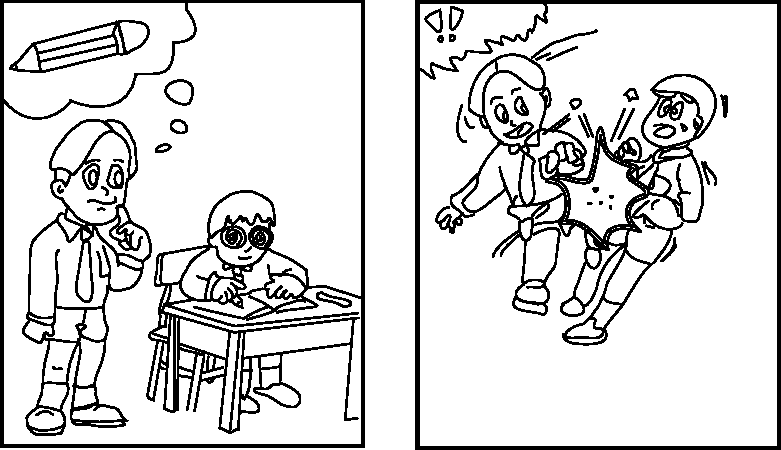
\includegraphics[width=\textwidth]{figures/comic.pdf}
\caption{Pictures taken from the cartoon oral production task used in \citet{Rose2000} (adapted).}
\label{fig:van:2}
\end{figure}

According to the authors, the methods should be refined through metapragmatic assessment or thinking/talking about their specific productions (p. 56). 

\citet{Cohen2003} applied the multiple-rejoinder DCT, which involved par\-ti\-ci\-pants reading not only the situations but also all of the replies. Twelve contexts were presented to the par\-ti\-ci\-pants, each of them requiring either a request or an apology. The context was introduced in English, but then the conversational replies were introduced in the language of the research site (see \REF{ex:van:7}, with replies in English as a matter of illustration). According to the authors, the multiple rejoinders aim to make the DCT “more reflective of the conversational turn-taking of natural speech” and should facilitate a more precise analysis of pragmatic language ability.


\ea%7
    \label{ex:van:7} 

         You completely forget a crucial meeting with the distinguished professor with whom you are doing an internship. An hour later you call him to apologize. The problem is that this is the second time you’ve forgotten such a meeting with your professor.   



Professor: What happened to you?


You: {\longrule}{\longrule}{\longrule}{\longrule}{\longrule}{\longrule}{\longrule}{\longrule}{\longrule}{\longrule}{\longrule}{\longrule}{\longrule}{\longrule}{\longrule}{\longrule}


Professor: I can imagine that you have a lot on your mind these days, but this is the second time you’ve missed a meeting you agreed to attend.


You: {\longrule}{\longrule}{\longrule}{\longrule}{\longrule}{\longrule}{\longrule}{\longrule}{\longrule}{\longrule}{\longrule}{\longrule}{\longrule}{\longrule}{\longrule}{\longrule}


Professor: Yes, indeed. I hope you won’t forget it next time.  


You: {\longrule}{\longrule}{\longrule}{\longrule}{\longrule}{\longrule}{\longrule}{\longrule}{\longrule}{\longrule}{\longrule}{\longrule}{\longrule}{\longrule}{\longrule}{\longrule}

Professor: I’m afraid I can’t reschedule it for today. Let’s try again next week at the same time.
    \z


A new tool, the Multimedia Elicitation Task (MET), was developed in \citet{Schauer2004} to investigate the acquisition of requests by German learners of English. This tool was designed to ensure comparable audiovisual contextual information for every participant. An introductory slide preceded each MET scenario telling par\-ti\-ci\-pants what would happen in the scenario (e.g. asking a professor to open a window, see \tabref{tab:van:2}). After 10 seconds, the actual scenario slide appeared providing par\-ti\-ci\-pants with audiovisual information, first in the form of a picture illustrating the situation and then as an audio description of the scenario (see \tabref{tab:van:2}). According to the author, the main methodological advantage of using the Multimedia Elicitation Task is that it allows comparability across various samples, while providing the researcher with the opportunity to use native speaker speech without the presence of an actual native speaker. Finally, in \citet{McLean2005}, after students were given an introduction about pragmatics in language learning, a set of DCTs were provided as the basis for group discussions about situations requiring the use of speech acts such as requests, apologies, and refusals. The main purpose of this activity was to encourage metapragmatic reflection, meaning to provide the students with an adequate context to think and talk about how language can or cannot be used in a variety of situations. The students were then asked to write personal DCTs for the class to discuss. 

\begin{table}
\begin{tabularx}{\textwidth}{p{.6\textwidth}Q}
\lsptoprule
 Visual input &  Audio input – Scenario 1 \\
 \midrule
 \vspace*{0pt}
 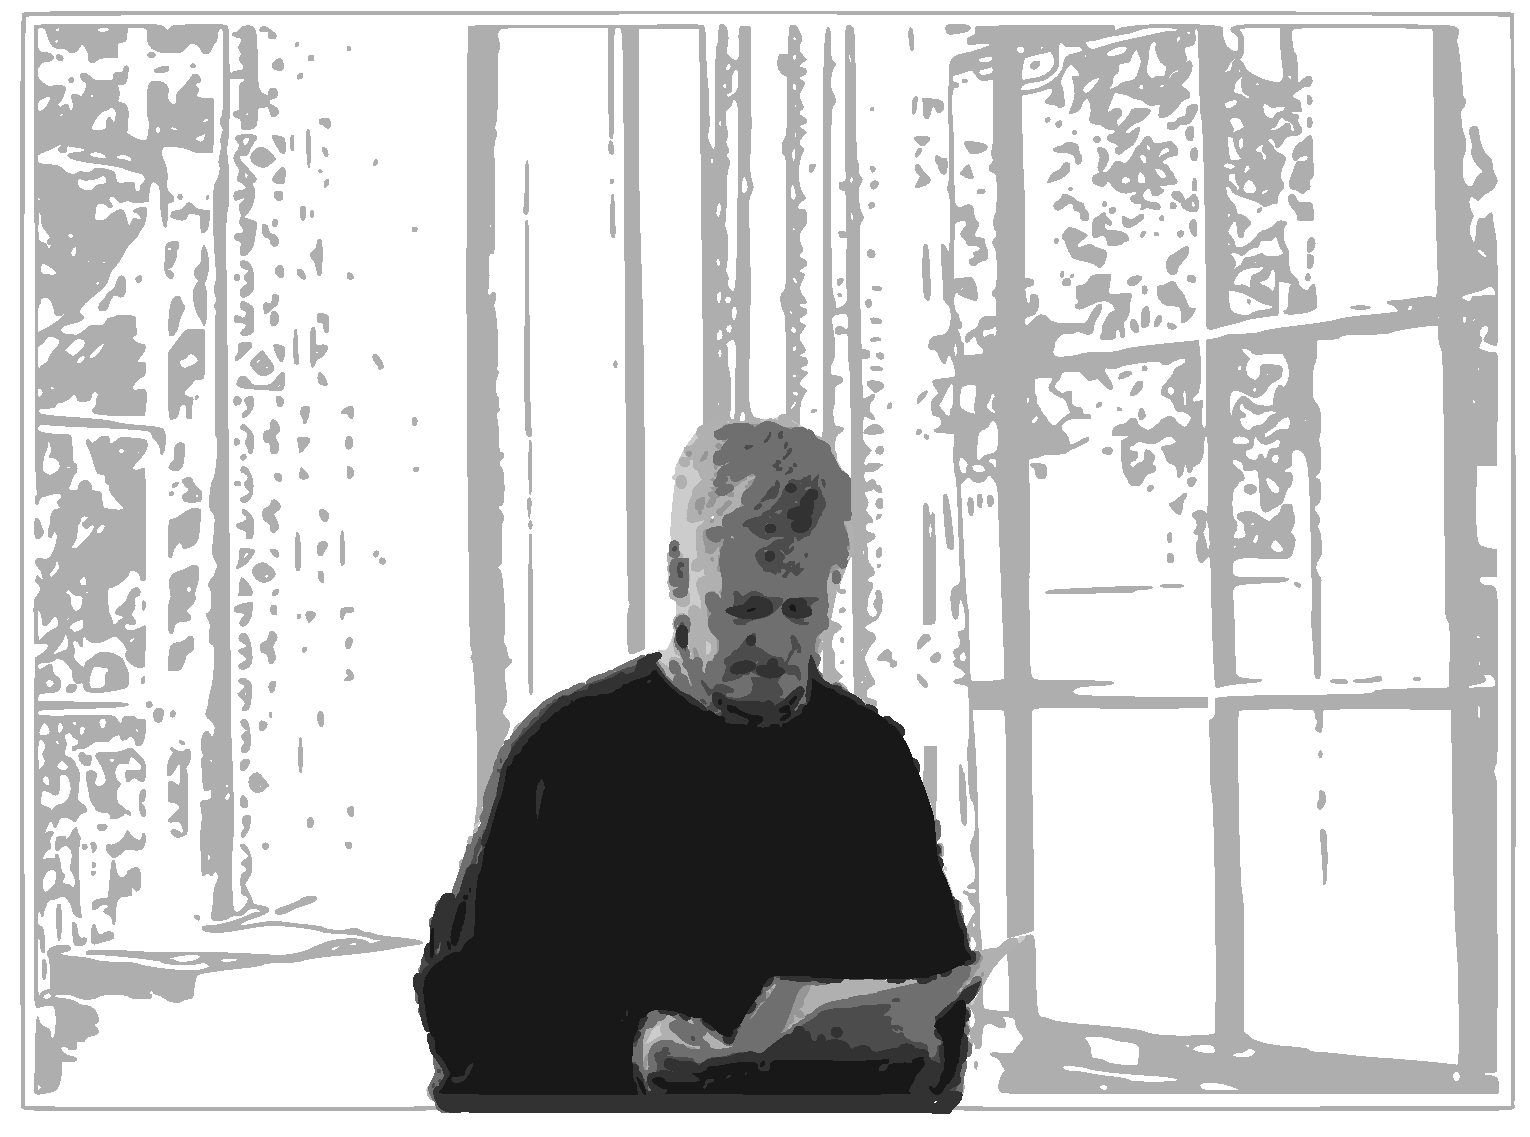
\includegraphics[width=.6\textwidth]{figures/readerphoto1.pdf}
 	  & \vspace*{0pt} You are attending a seminar. It is a very sunny day and the classroom is hot. The professor is standing near the window. You ask him to open it.\\
\lspbottomrule
\end{tabularx}
\caption{\label{tab:van:2} Scenario slide 1 for Scenario 1 taken from the MET task used in \citet{Schauer2004}.} 
Original picture can be found at \url{https://www.benjamins.com/#catalog/journals/eurosla.16/main}
\end{table}

\subsection{Proposals for improving the DCT in Romance prosody research}
\label{sec:van:3.2}
In this section we will address all of the weak points listed in \tabref{tab:van:1} and discuss the ways in which these potential problems can be circumvented. Then we will review some recent studies in which the design of the DCT differs from those versions introduced in \REF{ex:van:1}--\REF{ex:van:5} and discuss ways in which the authors address weaknesses of the general methodology used in prosody research.

To ensure that the scenarios are easy to understand, the context should be concise and the relevant information should be mentioned explicitly and not merely introduced in passing. In addition, the use of pictures to elicit information bears the risk of providing the speaker with obvious information. For this reason, using images should be avoided. However, when pictures shall be used, obviousness can be reduced or even avoided when the scenario is created in such a way that the test subject ‘thinks’ that s/he is the only one who sees the picture, while the (imagined) interlocutor does not.

In light of recent technical developments, one could imagine a completely new way to provide the test subjects with DCT scenarios: virtual reality (VR; see \citealt{Fox.2009} for details on VR).\footnote{We would like to thank A. Muntendam, p.c., for bringing up the idea of VR.} Using VR technologies, the test subject experiences a rich audiovisual context instead of a verbally presented scenario which depends on the imaginative powers of the researcher and the test subject. Let us imagine a DCT scenario evoking a \textit{first contact call}: the subject experiences herself entering a house, while the voice of a virtual narrator explains that she is entering the flat of her friend Maria. Being in the virtual house, the test subject sees that there is no one visible from the hall. The narrator asks her to call up to Maria, as she guesses that Maria is up in her room. After that, the test subject replies verbally as the scenario dictates. 
Previous psycholinguistic research has shown that VR creates an ecologically valid setting in which the test subject interacts with the virtual interlocutor in the way they would speak with human interlocutors (see \citealt{Heyselaar.2017,PEETERS.2017} and references cited therein). As in the typical DCT setting, the researcher still has control over the scenario with respect to pragmatic and politeness factors, stress patterns, etc. But VR, similarily to MET, additionally guarantees the repeatability of each scenario, since it does not depend on the quality of the involvement of the researcher – the virtual scenario is always the same. A crucial contrast to MET, however, is that VR provides the test subject with a complete audiovisual world with virtual agents and in which she does not see the laboratory surroundings. Even though using VR in linguistic research is relatively new, studies on speech rate and F0 (\citealt{Gijssels.2015,StaumCasasanto.2010}, respectively) show that VR can easily be used for prosodic research--a promising fact for virtual DCT scenarios.

As the intonational patterns obtained through this method may not always coincide with those previously found using other methodologies, we would like to point out that, while we understand the concerns, this does not necessarily imply that DCT is inadequate as a data collection instrument, but rather that we have elicited a wider or different set of patterns compared to previous research (in this sense we agree with Barbara Gili Fivela, personal communication, 02/2017).

As we saw in the previous section, the elicitation of speech acts is not always an easy task. We therefore recommend that the design of the contexts is carried out with care and attention to ensure that different speech acts are clearly differentiated. The full participation of the interviewer is fundamental; s/he should present the context in such a way that the participant feels immersed in the situation. If this is successful, the participant may confirm this feeling by smiling and nodding or, on the contrary, may make gestures of incomprehension (shoulder shrug, mouth turned down, etc.). Small adaptations of the situation to the context of the speaker (i.e. use of proper names of relatives/friends, specific places or festivals in the village/city, etc.) may be required and, as confirmed by \citet{Billmyer2000}, can lead to a more adequate participation.

Even when the contexts are carefully established, active directions may be needed to guide the recording process (such as asking the par\-ti\-ci\-pants to temporarily ignore certain culture-dependent rules). Potential problems could be avoided if the interviewer is a native speaker of the language/variety under study or if a native speaker is present during the recording session. Otherwise, the researchers should try to be familiar with culture-dependent rules of politeness or other psychological/social factors. Furthermore, attention should be paid to the participant recruitment process (see above). An alternative to the presence of a native speaker could be the use of the Multimedia Elicitation Task (see \citealt{Schauer2004}).

Previous proposals to strengthen the design of the DCT in Romance prosody research are rare and still very tentative. Recently, some studies have proposed modifications to the design of the DCT presented in \REF{ex:van:1}--\REF{ex:van:5} with the aim of overcoming existing limitations of the general methodology commonly used in prosody research (\citealt{ElviraGarcia2017,SanchezAlvarado.2018}). Other pro\-po\-sals do not improve the DCT itself, but rather propose complementing the DCT with additional tasks (a technique known as \textit{triangulation}), which can increase the validity/robustness of the results obtained through the DCT (\citeauthor{Vanrell2014evidentiality} \citeyear*{Vanrell2014evidentiality}; \citealt{Borras-Comes2015}). A study by Sánchez-Alvarado (under review) represents a new approach in the study of the prosody-information structure interface in Romance. So far, most of the research on this topic had made use of picture-based tasks to elicit different focus constructions (see \citealt{Gabriel2007,Muntendam2009,Vanrell2013catalanspanish,Feldhausen2014,FeldhausenVanrell2015}, among others). In her approach, Sánchez-Alvarado uses a contextualized sentence completion task based on the DCT. By using this technique, she aims to develop an elicitation method that can overcome one of the weaknesses of picture-based tasks, namely “the tendency shown by native speakers to respond with a single word” (\citealt{SanchezAlvarado.2018} citing \citealt{Ortega-Llebaria2014}). The questionnaire presented 25 items to 12 Asturian Spanish native speakers. Every context presented a scenario introducing an information gap to be filled by the participant (see \ref{ex:van:8}). Importantly, only one of the possible responses was presented to the par\-ti\-ci\-pants. This was done by creating three versions of the experiment. The prompt (such as \ref{ex:van:8}) was the same for each experiment, but the predetermined response varied (\ref{ex:van:8}a, \ref{ex:van:8}b, and \ref{ex:van:8}c respectively). Although this proposal clearly represents an improvement to the methods used to explore the prosody-information structure interface in Romance, it implies moving away from a core concept of the DCT: allowing the speaker to freely utter whatever response she deems appropriate as long as it fits the situation evoked by the prompt. Sánchez-Alvaro already restricts this freedom by providing the speaker with a set of answers (i.e. predetermined parts of possible answers) and as a consequence, the speaker is less free in his/her answers. In this way, the DCT no longer offers the possibility of giving a free response, which is one of the defining features of this method, as argued by \citet{Kwon2004}. 
 

\ea%8
    \label{ex:van:8} 

         \textit{Tu jefe te comenta que alguien pasó la noche en la oficina. No puedes ayudarle porque no sabes quién fue pero después, tu compañero te comenta que fue Andrea así que vuelves a la oficina del jefe y le dices...}

‘Your boss tells you that someone spent the night in the office. You cannot help him, because you do not know who it was but later your colleague tells you that it was Andrea, so you go back to the office and tell your boss?’

a. \textit{Andrea...}

b. \textit{Fue...} ‘It was’

c. \textit{Pasó la noche en la oficina...} ‘Spent the night at the office…’
\z

A similar modification in the design of the DCT is used in \citep{ElviraGarcia2017}, who analyze the prosody of semi-dependent and independent clauses with subordination marks in Peninsular Spanish (Castilian Spanish, Andalusian Spanish and the variety of Spanish spoken in Barcelona). A questionnaire with 123 items was presented to 10 native speakers of Peninsular Spanish. The variation in their DCTs consisted of providing not only a pragmatic context but also the lexical content of the utterance that par\-ti\-ci\-pants were requested to produce. To this end, each participant listened to the context, read the sentence appearing in the slide and, as soon as the slide disappeared, s/he performed a speech act including the given information and using the intonation the speaker would use in the same context (see \ref{ex:van:9}). As in the previous case, this approach has the advantage of eliciting very specific syntactic constructions (semi-dependent and independent clauses with subordination marks), while still controlling for the effects of pragmatic context. On the other hand, this proposal departs from the original idea of the DCT by weakening speakers’ freedom to answer in the way they would like. In conclusion, it is up to the researcher to decide what matters most: a careful control of the context and the syntactic structure of the target sentence, or that the speaker has the freedom to answer as s/he wishes. 

\ea%9
    \label{ex:van:9} 

         Imagine that we are talking about a common friend, Lorena. You know for sure that Lorena eats vegetables in the afternoon. Imagine that I ask you ‘‘Did you know that Lorena eats chocolate every afternoon?’’ 


[A PowerPoint slide appears on the screen with an image of a girl eating vegetables and the sentence \textit{¡Si merienda verdura!} ‘Yes she eats vegetables’]. 
    \z


\subsection{Proposals for complementing the DCT with further methods (triangulation)}
\label{sec:van:3.3}
Some proposals have been made towards the use of two or more methods (triangulation) to verify the validity of the data collected through DCT questionnaires while reducing possible task bias. For instance, \citet{Vanrell2014evidentiality} investigated the type of meaning encoded in yes-no questions through the combination of the question particle \textit{que} ‘that’ and the nuclear pattern L+H* L\% in Majorcan Catalan yes-no questions with the objective of understanding any temporal information related to this meaning. The DCT they created involved scenarios containing two evidential conditions ((i) inferred direct evidential and (ii) hearsay) and a non-evidential situation. Their questionnaire consisted of 12 situations, which were presented to 15 speakers. The results were quite convincing in showing that direct evidential contexts elicit the production of the L+H* L\% pattern headed by a question particle. Two additional experiments were carried out to further explore the degree of perceived appropriateness of the target intonational patterns to different pragmatic contexts as well as the information source at the time at which the evidence was available. The first additional experiment consisted of an acceptability task to rate the degree of appropriateness of the target intonational patterns to different evidential conditions. For the second additional experiment a multiple-choice questionnaire was created asking the subjects to answer two questions related to the information source (heard, seen, heard/seen, I don’t know) and the time of the evidence (just now, a few hours ago, yesterday, I don’t know). The results obtained through these three methods allowed the authors to conclude that three types of information are encoded in \textit{que}\_L+H* L\% questions: sentence modality, inference through direct evidence and immediate evidence \citep[1025]{Vanrell2014evidentiality}.

After the production experiment, \citet{Borras-Comes2015} also conducted a perception experiment based on the acceptability judgment task. Seventy-two speakers of Central Catalan were asked to rate the degree of adequacy between a vocative uttered with a specific intonational contour and its preceding discourse context. The results obtained in production were confirmed by those obtained in perception. Other proposals have been made in a more informal way. Andrea Pešková has indicated via personal communication (29.08.2016) that, in her experience, informants are able to correct/refine their own productions. Thus, a possible method to double-check the productions obtained through a DCT would be to use think-aloud protocols or some form of metapragmatic assessment. After being recorded answering to the DCT scenarios, par\-ti\-ci\-pants could listen to the utterances they produced in a second session and reflect on them.


\subsection{Summary}
\label{sec:van:4}

In the previous sections we have reviewed the weaknesses of the different DCT methods commonly used in prosodic research and we have discussed possible ways to strengthen them.  We offer a summary of these discussions in \tabref{tab:van:3}.

\begin{table}
\footnotesize
% \fittable{
\begin{tabularx}{\textwidth}{@{}p{4.5cm}X@{}}
\lsptoprule
 \bfseries Weaknesses & \bfseries Improvements\\
 \midrule
Scenarios that are natural and easy to understand are notoriously difficult to create. Difficulties in interpreting specific scenarios may lead to rising contours meaning “Did I do it well?” or to contours expressing obviousness. & Scenarios should be carefully crafted, the context should be brief but concise, and the relevant information should be explicitly mentioned so that no information is introduced merely in passing.
The use of images depicting information to be elicited should be very carefully crafted or avoided.
Using VR helps to create ecologically valid settings and might help to create authentic and understandable scenarios.
\\
\tablevspace
The intonational patterns obtained with this method may not always coincide with those described in previous studies. & (see discussion in \sectref{sec:van:2})\\
\tablevspace
Elicitation of less trivial speech acts can be difficult. & Care and attention are necessary in the design of the scenarios to ensure that the different speech acts are not mixed.
Involvement on the part of the interviewer and small adaptations should guarantee that the participant fully immerses herself in the task.
\\
\tablevspace
Cultural differences or social / psychological factors may arise. & Awareness on the part of the interviewer and readiness to intervene; for instance, asking the par\-ti\-ci\-pants to ignore certain culture-dependent conventions.\\
\tablevspace
The range of scenarios may not portray the variety of language uses in real situations. & This is a limitation in pragmatics but less so in prosodic research, where the focus lies on eliciting prototypical answers from a variety of speakers rather than on assessing the pragmatic repertoire of any given individual. \\
\tablevspace
Collecting the target sentences always implies a certain degree of free choice in the answers chosen by the speakers. The DCT does not allow for scripted speech (and thus cannot easily address research questions that need predetermined answers). & (see discussion in \sectref{sec:van:3.2})\\
\tablevspace
Each scenario allows for only one answer. & This problem could be circumvented by providing the speaker with different situations evoking the same communicative context. The speaker would have different tokens of the same context and can utter different answers. Alternatively, further methods can be used (triangulation).\\
\tablevspace
Setting up the different contexts might be difficult in cases in which the pragmatic differences between contexts are unclear. & A clear definition of the required speech acts is needed and the context should be carefully established according to these definitions. Pilot studies might help to figure out which contexts work well.\\
\lspbottomrule
\end{tabularx}
% }
\caption{\label{tab:van:3} Main weaknesses attributed to DCT used in the context of Romance prosody and proposals for how to address these issues.}
\end{table}

\section{Conclusions}

In this paper we have reviewed some studies that have applied the DCT to Romance prosody as a data collection instrument. We have concentrated on those studies that have addressed issues regarding the validity or reliability of the method as well as those that propose modifications to the design of the DCT. Our analysis has been organized according to the strengths and weaknesses identified by different scholars in applying this instrument to Romance prosody research. Finally, we have discussed the few studies that have used modified versions of the DCT design described in (\ref{ex:van:1}--\ref{ex:van:5}) or have added supplementary tasks.

All of the studies discussed in this chapter confirm that some of the strengths of the DCT lie in its flexibility and adequacy for: 1) obtaining semi-spontaneous speech within a short period of time, 2) eliciting comparable spontaneous data across speakers and varieties, 3) working with older and illiterate people, 4) requiring little and easily transportable equipment, 5) controlling both the context (pragmatic and politeness factors) and the target sentence (stress pattern, sentence type and segmental and syntactic structure), 6) easily addressing interface phenomena, 7) being feasible for monolingual and bilingual speakers, and 
8) allowing spontaneity in the responses. 


Despite these considerable strengths, attention should be devoted to the following possible drawbacks: 1) the fact that some speakers may not understand the task, leading to the appearance of rising contours meaning “Did I do it well?” and/or expressing obviousness, 2) the intonational patterns found may not always coincide with previous investigations using a different methodology, 3) the elicitation of less trivial speech acts can be a difficult task, 4) cultural differences or psychological/social factors may arise, 5) the range of situations can be limited and may not portray the richness of language uses in real situations, 6) collecting the target sentences always implies a free choice in the answers, 7) each context allows for only one answer and, for that reason, this method does not allow to assess the felicity of other possibilities realized in the same context, and 8) setting up the different contexts may be challenging.


In the present chapter we have also proposed some improvements to ameliorate the weaknesses we have named. These include the following: 1) the scenarios should be carefully crafted, the context should be brief and concise and the use of images depicting the information to be elicited should be avoided, 2) special effort should be invested so that the participant feels immersed in the task, 3) the interviewer should be aware that cultural or social/psychological differences may arise and should be ready to intervene when necessary, 4) triangulation should be considered as a way to reduce possible task bias, and 5) the different speech acts should be clearly defined.

We believe that the DCT is definitely an adequate method for eliciting features such as pitch and intonation (contrary to what had been argued in \citealt{Kasper2000}), although further research is needed to directly address the validity/reliability of the method in prosody research. In the words of Lusia M. Nurani: “The investigation of the DCT’s design will bring about a reassessment of instrument design which will lead to the improvement to the usefulness of DCT”\citep[676]{Nurani2009}. This applies not only to research in pragmatics, but is also particularly relevant for research in prosody as well as for advancing the field of language testing in general. 


\section*{Acknowledgments}

This paper has benefited from the comments offered by the par\-ti\-ci\-pants in a session created in Academia.edu. We are grateful to the par\-ti\-ci\-pants (Marco Barone, Ander Egurtzegi, Wendy Elvira-García, Barbara Gili Fivela, Guillermo González Campos, Andrea Pešková, Melanie Uth) for the time devoted to reading and discussing our manuscript. Our gratitude also goes to the par\-ti\-ci\-pants of the session on “Prosody and Conceptual Variation” at the 35\textsuperscript{th} Romanistentag – the biannual conference of the German Society of Romance Philology (Zürich, 8--12 October 2017) for their important comments and remarks. The second author would also like to thank the students of his class on intonation in Spanish (summer term 2016) for their feedback on the method. Our further gratitude goes to Julia Otto, the student assistant of the second author, for her help with the references. This research has been partially funded by the Spanish government via projects FFI2016-76245-C3-1-P and FFI2017-87699-P (Ministerio de Economía, Industria y Competitividad). We would also like to thank the two anonymous reviewers for their valuable comments for improving the quality of the paper. All errors are our own.

{\sloppy
\printbibliography[heading=subbibliography,notkeyword=this]
}



\end{document}


